%%% Template originaly created by Karol Kozioł (mail@karol-koziol.net) and modified for ShareLaTeX use

\documentclass[a4paper,11pt]{article}

\usepackage[T1]{fontenc}
\usepackage[utf8]{inputenc}
\usepackage{graphicx}
\usepackage{xcolor}
\usepackage[export]{adjustbox}

\renewcommand\familydefault{\sfdefault}
\usepackage{tgheros}
\usepackage{droidsansmono}

\usepackage{amsmath,amssymb,amsthm,textcomp}
\usepackage{enumerate}
\usepackage{multicol}
\usepackage{tikz}

\usepackage{geometry}
\geometry{left=25mm,right=25mm,%
bindingoffset=0mm, top=20mm,bottom=20mm}


\linespread{1.3}

\newcommand{\linia}{\rule{\linewidth}{0.5pt}}

% custom theorems if needed
\newtheoremstyle{mytheor}
    {1ex}{1ex}{\normalfont}{0pt}{\scshape}{.}{1ex}
    {{\thmname{#1 }}{\thmnumber{#2}}{\thmnote{ (#3)}}}

\theoremstyle{mytheor}
\newtheorem{defi}{Definition}

% my own titles
\makeatletter
\renewcommand{\maketitle}{
\begin{center}
\vspace{2ex}
{\huge \textsc{\@title}}
\vspace{1ex}
\\
\linia\\
\@date \hfill
\@author
\vspace{4ex}
\end{center}
}
\makeatother
%%%

% custom footers and headers
\usepackage{fancyhdr}
\pagestyle{fancy}
\lhead{}
\chead{}
\rhead{}
\lfoot{Assignment 1}
\cfoot{}
\rfoot{Page \thepage}
\renewcommand{\headrulewidth}{0pt}
\renewcommand{\footrulewidth}{0pt}
%

% code listing settings
\usepackage{listings}
\usepackage[space=true]{accsupp}

\definecolor{codegreen}{rgb}{0,0.6,0}
\definecolor{codegray}{rgb}{0.5,0.5,0.5}
\definecolor{inlinecode}{rgb}{0.3,0.3,0.3}
\definecolor{codepurple}{rgb}{0.58,0,0.82}
\definecolor{backcolour}{rgb}{0.95,0.95,0.92}
\lstset{
    language=C,
    basicstyle=\ttfamily\small,
    aboveskip={1.0\baselineskip},
    breakatwhitespace=false,         
    keepspaces=true,
    belowskip={1.0\baselineskip},
    columns=fullflexible,
    extendedchars=true,
    breaklines=true,
    tabsize=4,
    prebreak=\raisebox{0ex}[0ex][0ex]{\ensuremath{\hookleftarrow}},
    frame=lines,
    showtabs=false,
    showspaces=false,
    showstringspaces=false,
    commentstyle=\color{codegreen},
    keywordstyle=\color{magenta},
    numberstyle=\tiny\color{codegray},
    stringstyle=\color{codepurple},
    numbers=left,
    numberstyle=\small\noncopynumber,
    stepnumber=1,
    numbersep=10pt,
    captionpos=t,
    escapeinside={\%*}{*)}
}

\newcommand{\noncopynumber}[1]{
    \BeginAccSupp{method=escape,ActualText={}}
    #1
    \EndAccSupp{}
}

%%%----------%%%----------%%%----------%%%----------%%%

\begin{document}

\title{CSE-016 Programming Lab Assignment \textnumero{} 1}

\date{02/03/2024}

\author{Youssef Ahmed Samy Kassem\\ \hfill ID 9545 -- Group 3 -- Lab 1\\ \hfill SSP -- Faculty of Engineering, Alexandria University\\}


\maketitle
\textit{Document structure is detailed in the final page.}
\section{Problem}
\textbf{Problem (C):} Take Home Assignment: Write a program that prints the following shape:\\
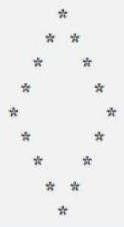
\includegraphics[width=0.1\textwidth, center]{image.png}

\section{Student's Solution}
\subsection{Source Code}
\begin{lstlisting}[label={list:first},title=Program's \texttt{\color{inlinecode}{main.c}} File -- Uses \texttt{\color{inlinecode}{printf()}} to output a line-by-line representation of the polygon.]
#include <stdio.h>
#include <stdlib.h>

int main()
{
    printf("    *    \n");
    printf("   * *   \n");
    printf("  *   *  \n");
    printf(" *     * \n");
    printf("*       *\n");
    printf(" *     * \n");
    printf("  *   *  \n");
    printf("   * *   \n");
    printf("    *    \n");
    return 0;
}
\end{lstlisting}
\subsection{Output}
\begin{lstlisting}[language=Tex,numbers=none,label={list:second},title=Program's output to console -- in plaintext.]
    *
   * *
  *   *
 *     *
*       *
 *     *
  *   *
   * *
    *

Process returned 0 (0x0)   execution time : 0.012 s
Press any key to continue.
\end{lstlisting}
\subsection{Evidence of Work (Screenshots)}
A. Desktop Screenshot\\\\
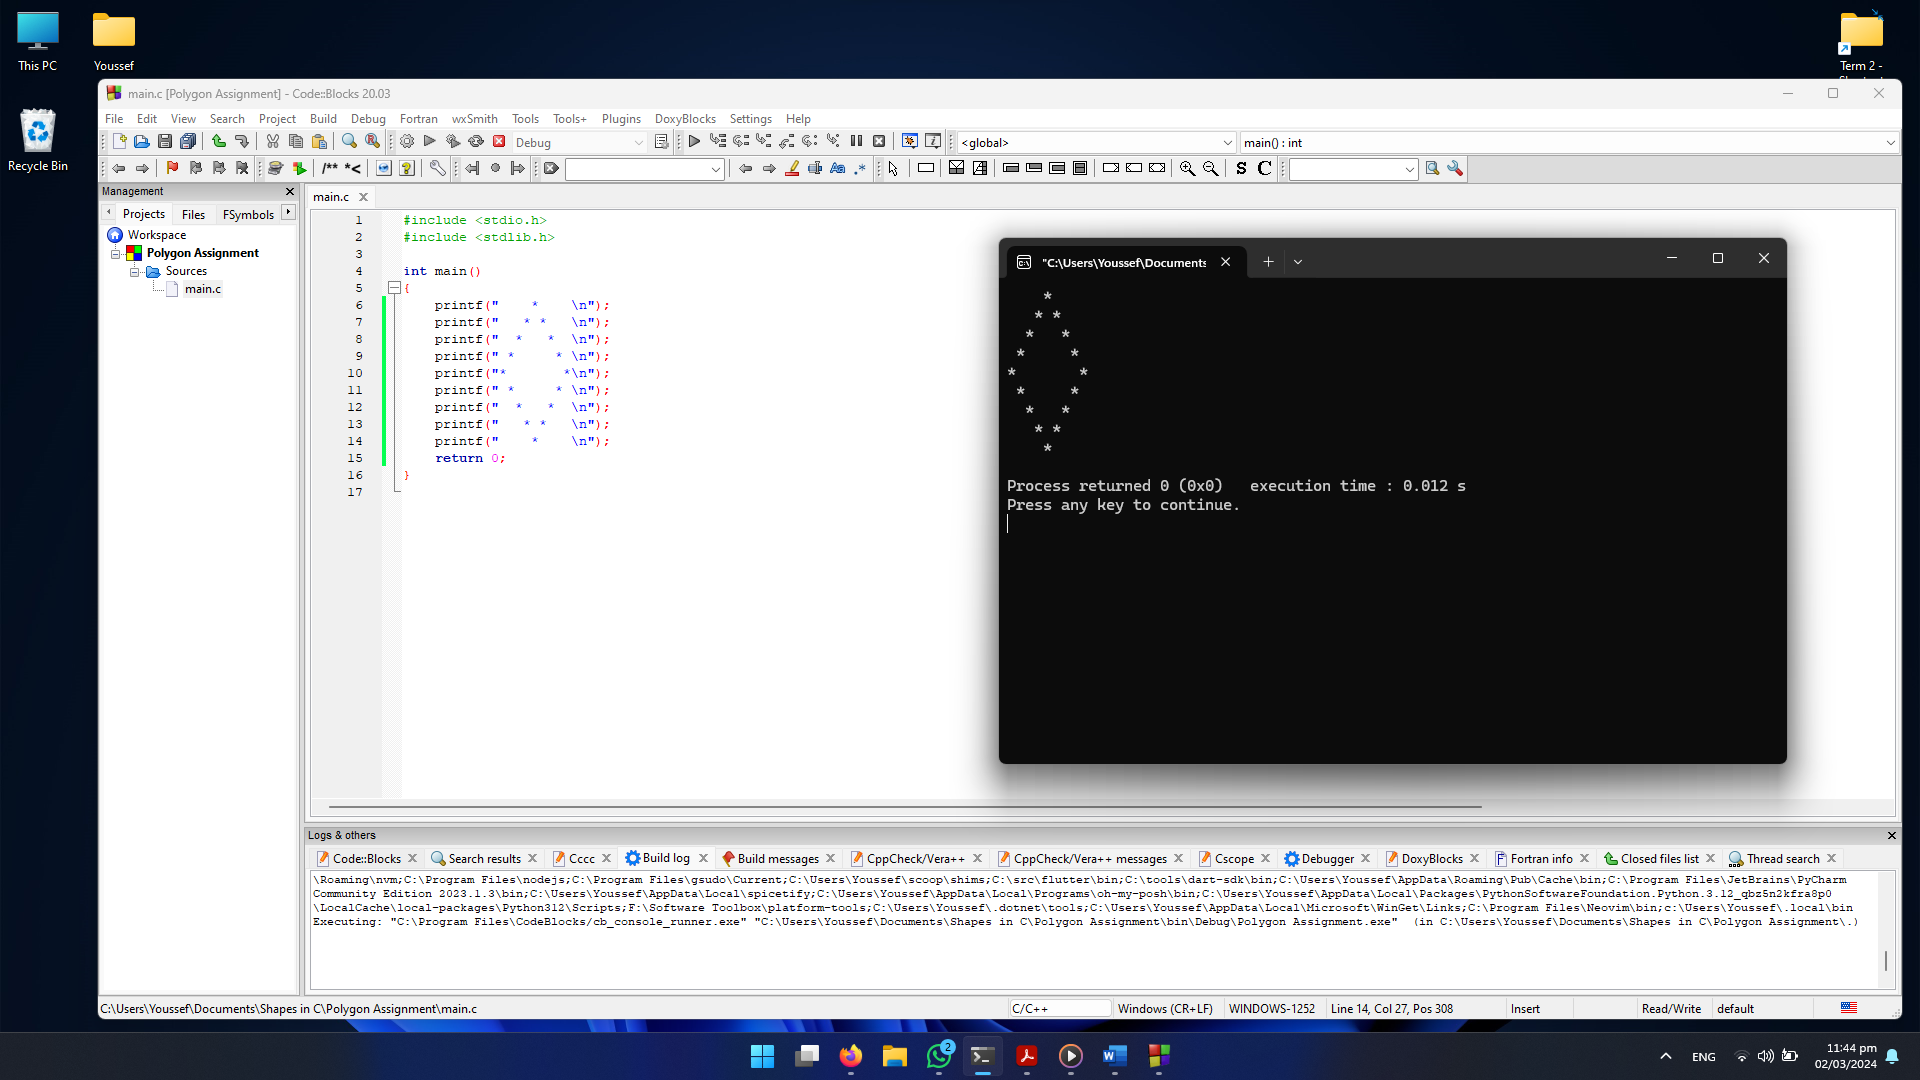
\includegraphics[width=1.1\linewidth, center]{desktop.png}
\newpage
B. Codeblocks IDE Screenshot\\\\
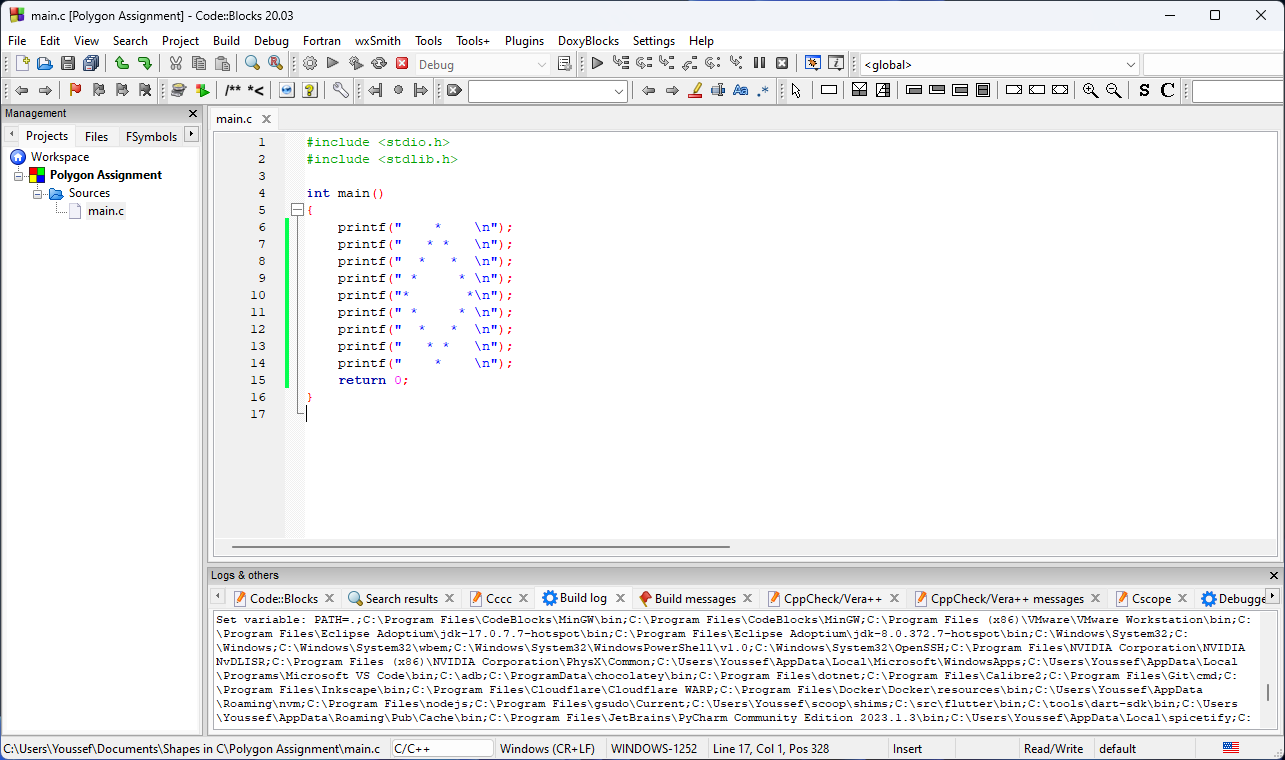
\includegraphics[width=1.1\linewidth, center]{codeblocks.png}
C. Output in Console Terminal Screenshot\\\\
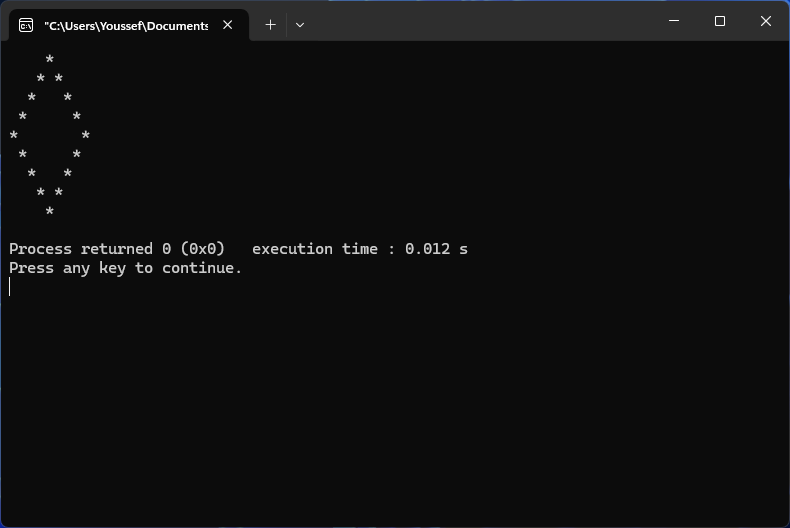
\includegraphics[width=1.1\linewidth, center]{terminal.png}

\subsection{Documentation}
\subsubsection{Specifications}
\begin{itemize}
    \item \textbf{Dependencies:}
    \begin{itemize}
        \item \texttt{\color{inlinecode}{stdio.h}} header file, part of the C Standard Library (Required)
        \item \texttt{\color{inlinecode}{stdlib.h}} (Unused)
    \end{itemize}
    \item \textbf{Compiler:} GNU C Compiler \texttt{\color{inlinecode}{(gcc)}} version 8.1.0
    \item \textbf{Unit Testing:} not applicable
    \item \textbf{Supported Platforms:} OS: (any), architecture: (any)
    \item \textbf{Tested On:}
    \begin{itemize}
        \item Windows 11, x64\_86 or x64 arch
    \end{itemize}
\end{itemize}
\subsubsection{Troubleshooting \& Misc}
\textit{Line 2} is included by default, we were not instructed to omit it.\\
\textit{Line 15} return codes are usually only useful on Unix-like environments, we were not instructed to omit it.
\subsection{License \& Warranty}
Any source code or compiled application included or distributed by the author (Youssef Ahmed Samy) is licensed under the Lesser GNU Public License (LGPL) when applicable, excluding instances where the source code or program function is too generic -- like in "Hello World" programs.\\
\textbf{THE SOFTWARE INCLUDED HEREBY IS PROVIDED WITHOUT EXPLICIT OR IMPLIED WARRANTY, THE AUTHOR IS ABSOLVED OF ANY CONSEQUENCES OF MISUSING OR IMPROPERLY HANDLING THE CODE OR PROGRAM.}
\tableofcontents
\end{document}
